%%%%%%%%%%%%%%%%%%%%%%%%%%%%%%%%%%%%%%%%%%%%%%%%%%%%%%%%%%%%%%%%%%%%%%%%%%%
%%%                                                                     %%%
%%%   LaTeX template voor het verslag van P&O: Computerwetenschappen.   %%%
%%%                                                                     %%%
%%%   Opties:                                                           %%%
%%%     tt      Tussentijdsverslag                                      %%%
%%%     eind    Eindverslag                                             %%%
%%%                                                                     %%%
%%%   4 november 2013                                                   %%%
%%%   Versie 1.1                                                        %%%
%%%                                                                     %%%
%%%%%%%%%%%%%%%%%%%%%%%%%%%%%%%%%%%%%%%%%%%%%%%%%%%%%%%%%%%%%%%%%%%%%%%%%%%

\documentclass[eind]{penoverslag}

%%% PACKAGES %%%
\usepackage{graphicx}
\setlength\parindent{0pt}

\begin{document}

% == TITELPAGINA == %
\team{Indigo} % teamkleur
\members{\\
        Wander Bavin\\
        Vince Goossens\\
        Dimitri Jonckers\\
        Sunil Tandan\\
		Wout Vekemans\\} % teamleden
\maketitlepage


% == SAMENVATTING == %
\begin{abstract}
\noindent
TODO!!!!!! uitbreiden\\
Dit document bespreekt de autonome zeppelin van Team Indigo, gemaakt in het kader van P&O Computerwetenschappen. Deze zeppelin, gebouwd met 2 ballonnen en 3 motoren en aangestuurd door een Raspberry Pi, kan commando's uitvoeren die op QR-cedes staan.\\
Dit verslag documenteert onze bevindingen en vooruitgang. Meer concreet beschrijven we de opbouw van onze zeppelin en de structuur van de software.
\end{abstract}


% == INHOUDSOPGAVE == %
\tableofcontents\newpage


% == INLEIDING == %
\section{Inleiding}
Het doel van deze opdracht is een autonome zeppelin te ontwikkelen. De zeppelin wordt aangestuurd door een Raspberry Pi. Via QR-codes kunnen instructies gegeven worden, zoals ``stijg 50cm'' of ``draai 45   graden''. De gebruiker kan via een GUI op een client-pc zelf de pijltjestoetsen gebruiken om de zeppelin aan te sturen of gegevens bekijken over de toestand van de zeppelin (bijvoorbeeld de huidige hoogte).

\paragraph{Fysisch ontwerp}
~\\ 
De zeppelin bestaat uit een houten frame waaraan 2 grote ronde heliumballonnen vastgemaakt zijn. Aan het frame is een afstandssensor gekoppeld die naar onderen is gericht. Verder is er een camera naar beneden gericht. Zowel de camera als de afstandssensor zijn verbonden met de Raspberry Pi die in het frame zit ingebed. Het geheel bevat drie propellers: twee voor horizontale bewegingen en \'{e}\'{e}n voor verticale bewegingen.


\paragraph{Software ontwerp}
~\\
Het grootste deel van de opdracht is het schrijven van de software in een taal naar keuze. Wij hebben gekozen voor Java. De software bestaat uit 3 grote delen: de GUI, de communicatie tussen GUI en Raspberry Pi en de interne programmatie op de Pi (Zie figuur \ref{schema}). \\
De communicatie tussen GUI en de Raspberry Pi gebeurt via sockets. Hierbij worden objecten uitgewisseld tussen de client en de server (de Pi), die commando's doorgeven aan de zeppelin of de status doorgeven aan de gebruiker. De interne programmatie op de Pi moet op basis van gegevens van zijn sensoren en instructies van QR-codes (en commando's van de gebruiker) de motoren aansturen. 

\begin{figure}[ht!]
\centering
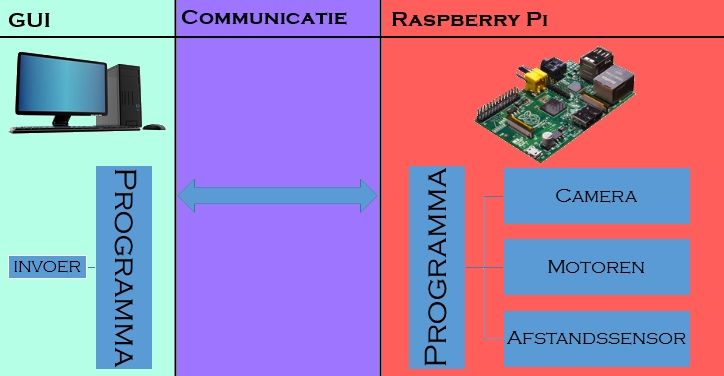
\includegraphics[height=55mm]{Schema.jpg}
\caption{Architectuur}
\label{schema}
\end{figure}


% == Beschrijving materiaal en bouw zeppelin == %
\section{Beschrijving materiaal en bouw zeppelin}
De zeppelin bestaat uit een frame waaraan alle onderdelen zijn vastgemaakt. Hierop worden onder andere 3 propellers bevestigd. Twee hiervan dienen om naar links en rechts te draaien. Om vooruit te bewegen worden deze samen geactiveerd met dezelfde kracht. Deze propellers bevinden zich aan de uiteindes van de vleugels. De derde propeller, om de zeppelin te laten stijgen, is naar beneden gericht. De propellers kunnen op volle kracht worden aangestuurd (in 2 richtingen) of door middel van pwm\footnote{en.wikipedia.org/wiki/Pulse-width\_modulation}. Door pwm is het mogelijk om naast de richting ook de kracht van de motor in te stellen.~\\
TODO afbeelding frame

Om het geheel in de lucht te houden, zitten er 2 heliumballonnen (ongeveer 90cm diameter) vast aan de bovenkant van het frame. \\
\\
De zeppelin wordt aangestuurd door een Raspberry Pi model A (zie Figuur \ref{Pi}). Deze heeft volgende specificaties: 
\begin{itemize}
	\item \emph{Processor:} 700MHz ARM
	\item \emph{Geheugen:} 256MB 
	\item \emph{Poorten:} 1 USB 2.0, HDMI, audio out, RCA video
	\item \emph{Voeding:} Micro USB
	\item GPIO-pinnen om de hardware aan te sturen
\end{itemize}

\begin{figure}[ht!]
\centering
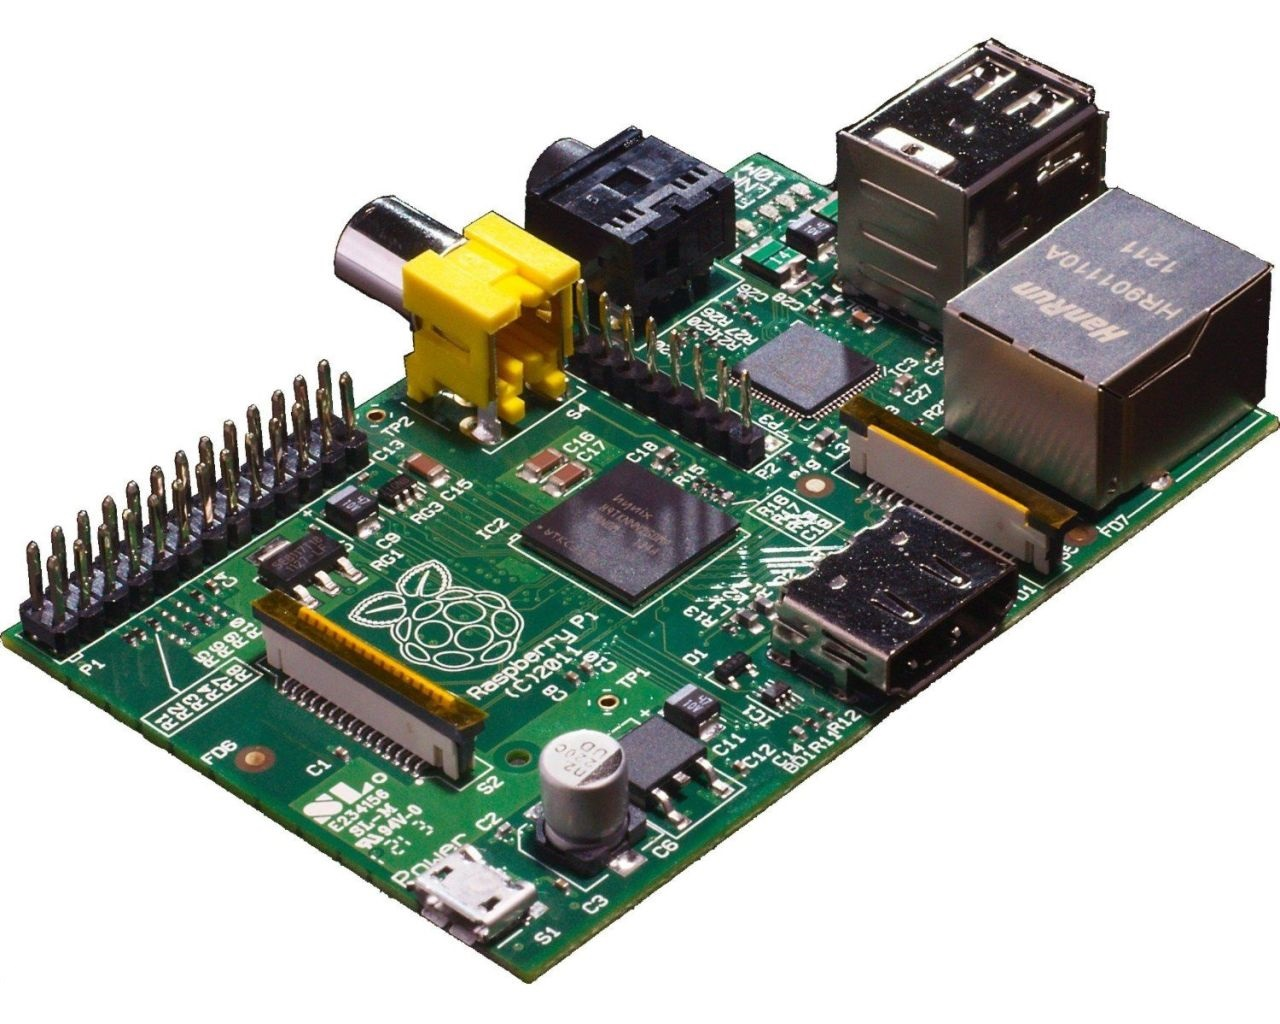
\includegraphics[height=30mm]{raspb.jpg}
\caption{Raspberry Pi}
\label{Pi}
\end{figure}

In de Raspberry Pi zit een SD-kaart van 4 GB. Hierop staat Raspbian, het standaard besturingssysteem van de Raspberry Pi. \\

Verder zijn er nog 2 devices waarvan de zeppelin gebruik maakt:
\begin{itemize}
	\item De camera laat toe foto's te nemen met een maximum resolutie van 5 MP. Hiermee kunnen we onder andere beelden maken van QR-codes. Daarnaast kan de camera video's maken met resoluties tot 1080p. 
	\item De afstandssensor kan worden gebruikt om met ultrasone trillingen de afstand te meten tussen de zeppelin en de grond of muur. Het bereik gaat van 2-400 cm. \\
\end{itemize}

\\

TODO zeppelin figuur

Om het geheel te monteren, hebben we gebruik gemaakt van plakband en zipties (bundelbandjes). 



% == Testen == %
\section{Testen}

Om er zeker van te kunnen zijn dat het aansturen van de zeppelin correct gebeurt, is het nodig dat de componenten getest worden. In de volgende sectie volgt hierover meer informatie. \\
\subsection{Afstandssensor}

In deze sectie gaan we dieper in op de testen die we gedaan hebben naar de nauwkeurigheid en snelheid van de afstandssensor.

\paragraph{Opstelling} ~\\ 
Benodigdheden:
\begin{itemize}
	\item RaspberryPi met afstandssensor
	\item houten scherm
	\item meetlat
\end{itemize}
Deze componenten worden in deze opstelling geplaatst : zie figuur \ref{opstelling}
\begin{figure}[ht!]%
\centering
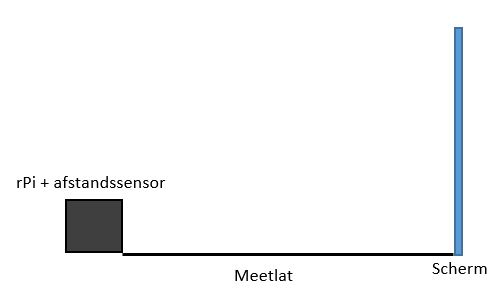
\includegraphics[scale=0.6]{opstelling.jpg}%
\caption{testopsteling}%
\label{opstelling}%
\end{figure}

\paragraph{Verloop} ~\\ 
De test bestaat uit het meten van 11 verschillende afstanden (10, 20, 30, 60, 90, 100, 110, 120, 130, 140 en 150 cm). Deze zijn zo gekozen om informatie te hebben over voldoende punten binnen het vlieghoogtebereik. Deze afstanden worden elk 500 keer gemeten, om de 60 ms. Deze waarden zijn zo gekozen, om toch voldoende nauwkeurigheid te hebben, veronderstellende dat er uitschieters zouden zijn.

\paragraph{Gegevens en verwerking} ~\\ 
Het uitvoeren van de testen nam per afstand gemiddeld 32 seconden in beslag. Omdat dit tijdens het opereren van de zeppelin onhaalbaar is, hebben we besloten om het interval te verkleinen. Zo kunnen de metingen sneller gebeuren. Hiervoor hebben we een extra test uitgevoerd op een hoogte van 170cm. Het blijkt dat we het interval tussen metingen kunnen terugbrengen naar 20 ms. Bij lagere waardes gaan signalen door elkaar lopen en zo de meting verstoren. \\

We hebben d.m.v. rolling median de mediaan berekend van 10 en 20 opeenvolgende gegevens, uit de set van 500 waardes per hoogte. Minder dan 10 is niet nauwkeurig genoeg, en voor meer dan 20 samples is de registratietijd te hoog. Uit deze gegevens hebben we om een aantal redenen besloten om een window van 10 samples te nemen.  Ten eerste is er de nauwkeurigheid als de zeppelin stijgt/daalt. Het hoogteverschil tussen sample 1 en 10 is immers kleiner dan dat tussen 1 en 20. Ten tweede is er de snelheid. Het spreekt voor zich dat het registreren van 10 samples minder lang duurt dan 20 samples. Tenslotte is er ook het minieme verschil tussen de gemiddelde mediaan bij 10 en 20 metingen. Minder metingen zorgen dus voor een even grote nauwkeurigheid. 

Een nadeel is wel dat de standaardafwijking van de medianen bij een breedte van 10 samples gemiddeld 0.2 cm groter is dan bij 20 samples. Dit weegt echter niet op tegen de winst aan snelheid en nauwkeurigheid.\\ 

Voor de meetgegevens: zie onderstaande tabel. \\

\begin{tabular}{r||r|r|r|r|r|r|r|r|r|r|r}
\textbf{Afstand} & 10 & 20 & 30 & 60 & 90 & 100 & 110 & 120 & 130 & 140 & 150 \\
\hline \hline 
$\mu$ (med.) (10) & 10.8 & 20.5 & 30.8 & 58.0 & 88.3 & 98.7 & 108.5 & 117.3 & 127.74 & 137.0 & 147.10 \\
$\mu$ (med.) (20) & 10.8 & 20.7 & 30.7 & 58.0 & 88.3 & 98.7 & 108.5 & 117.3 & 127.7 & 137.0 & 147.1 \\
$\sigma$ (med.) (10) & 0.21 & 0.52 & 0.82 & 0.55 & 0.70 & 0.72 & 0.68 & 0.94 & 0.58 & 0.60 & 0.69 \\
$\sigma$ (med.) (20)& 0.09 & 0.33 & 0.71 & 0.41 & 0.59 & 0.56 & 0.47 & 0.54 & 0.43 & 0.37 & 0.49 \\
\end{tabular}

\paragraph{Conclusie} ~\\ 
De afstandsmeter meet het meest nauwkeurig bij kleine afstanden, bij grotere afstanden (meer dan 60 cm) liggen de meetresultaten gemiddeld iets onder de werkelijke afstand. Relatief gezien blijft de fout nog klein en kunnen we deze afwijking in het vervolg incalculeren bij het bepalen van de meetwaarden. De afstandssensor geeft telkens de mediaan van 10 gegevens door volgens het principe van de “rolling median”-techniek. Tien gegevens zorgen voor voldoende nauwkeurigheid, maar hebben ook het aspect dat de mediaanberekeningen snel genoeg gebeuren. Tevens is dit bij een hoogteverandering accurater. Deze methode boet wel in op de standaardafwijking. De gegevens wijken dus meer uit, maar dit weegt niet op tegen de voorgenoemde pluspunten. Om de afstandsregistratie nog sneller te laten verlopen, meet de afstandsmeter om de 20 ms.

\subsection{Camera}

\textbf{Deze test is nog niet uitgevoerd.} \\
TODO
Het testen van de camera lijkt op het eerste zicht eenvoudig, maar er komt veel meer bij kijken dan enkel foto's nemen. Er moet rekening gehouden worden met lichtintensiteit, responstijd van de camera, positie van de QR-code op de foto, \ldots \\

De lichtintensiteit wordt getest in een kamer met controleerbare lichtbron (d.m.v. lichtschakelaar, verduistering). Er wordt getest hoe licht het moet zijn in de kamer opdat de QR-code in de foto nog herkend wordt door het programma. \\

We hebben al kleine testen uitgevoerd waarin de QR-code lichtjes gedraaid was (invalshoek), en er was geen probleem om ze te lezen. Omdat de QR-code altijd recht onder de zeppelin zal staan, gaan we dit niet verder testen. \\

De responstijd (tijd tot herkennen QR-code) wordt getest door in verschillende omstandigheden een code te fotograferen. Een simpel printcommando in Java vertelt ons hoe lang het verwerken duurt. Hiervoor wordt de interne klok van de computer gebruikt. Om een globaal beeld te krijgen van de responstijd wordt een gemiddelde berekend van deze gegevens. We verwachten dat op grotere hoogtes (grotere afstand tot de code) we een afbeelding moeten nemen in hogere resolutie, waardoor de verwerkingstijd langer zal zijn. \\

Om te bepalen tot op welke afstand de camera foto's kan maken die herkend kunnen worden, is er een eenvoudige test: de camera fotografeert een QR-code vanop verschillende afstanden. 
De positie van de QR-code in de foto is een cruciaal element. De codes bevatten commando’s die relatief ten opzichte van de huidige positie moeten worden uitgevoerd. Kleine afwijkingen van de positie van de code tot het midden van de foto zijn onvermijdelijk en zullen zich voortplanten tijdens het verderzetten van het parcours. Dit heeft echter meer betrekking tot het testen en calibreren van de motoren (zie verder). \\


\subsection{Motoren}
\textbf{Deze test is nog niet uitgevoerd.} \\

We zijn bij onze eerste experimenten al enkele zaken te weten gekomen. Zo blijkt dat een minimale pwm-waarde van ongeveer 740 nodig is (ter info: maximumwaarde is 1024) om de propeller in beweging te krijgen. Daarnaast hebben we al gezien dat wanneer je de motoren voor enkele seconden laat draaien, de zeppelin nog een vrij lange tijd gaat uitbollen. \\

Hieronder is meer informatie te vinden over hoe we concreter en grondiger gaan testen voor bepaalde bewegingen. \\

\paragraph{Zijwaartse bewegingen} ~\\ 
Om de zijwaartse bewegingen te testen, gaan we kijken hoe lang we de motor moeten aanzetten om een hoek van 10$^\circ$ , 20$^\circ$, 30$^\circ$, \ldots uit te voeren. We zullen deze testen uitvoeren op hoeken naar links. Hiervoor zetten we de linkermotor op volle kracht achteruit en de rechtermotor op volle kracht vooruit. \\

Om dit te testen, gaan we de zeppelin moeten positioneren boven een soort 'roos': een cirkel waarop de graden staan aangeduid. Aan de hand van foto's van de naar onder gerichte camera, kunnen we dan manueel aflezen hoe ver de zeppelin gedraaid is. \\

Indien we deze gegevens voor hoeken van 10 tot 180 graden hebben, kunnen we deze plotten. Hier verwachten we een lineair patroon te zien vanaf een bepaalde hoek, namelijk bij de hoek waarbij de maximale kracht van de motor bereikt is. Het lineair patroon gaat doorbroken worden wanneer de gevraagde hoek bijna is bereikt. \\

Wanneer we deze functie gevonden hebben, zijn enkel de volgende gegevens nodig:
\begin{itemize}
	\item data voor voldoende hoeken kleiner dan de kritieke hoek waarbij het maximumvermogen van de motor wordt bereikt
	\item de lineaire functie
	\item duur van uitbollen
\end{itemize}
Voor kleine hoeken kunnen we dan een soort van tabel raadplegen, voor hoeken groter dan de kritieke hoek gebruiken we de lineaire functie. \\

Als laatste moeten we controleren of deze gegevens hetzelfde zijn voor bewegingen naar de rechterkant.  Dit doen we door dezelfde gegevens voor een aantal hoeken toe te passen. \\

\paragraph{Voorwaartse bewegingen} ~\\ 
Om voorwaartse bewegingen uit te voeren, zetten we zowel linker als rechter motor aan. Uit de testen die we gedaan hebben bij zijwaartse bewegingen, weten we of de 2 motoren hetzelfde afgesteld zijn. Indien ze niet perfect afgesteld zijn, zullen we moeten testen hoe vaak we tijdelijk de krachtigste motor moeten uitschakelen om een zo perfect mogelijke rechte baan te bekomen. \\

Het testen van de voorwaartse beweging gaat heel gelijkaardig zijn aan het testen van de zijwaartse bewegingen.  De zeppelin beweegt boven een liniaal.  Aan de hand van foto's van de camera kunnen we zien hoever hij van de rechte lijn afgeweken is en hoever hij geraakt is. We gaan opnieuw kunnen afleiden na hoeveel tijd de zeppelin zijn maximum vermogen bereikt. Zo gaan we opnieuw een formule opstellen die we dan gebruiken om te bepalen hoe lang we de motoren moeten laten draaien om een bepaalde afstand af te leggen. \\

\paragraph{Verticale bewegingen} ~\\ 
We gaan allereerst op zoek naar de juiste pwm waarde waarbij de zeppelin op dezelfde hoogte blijft zweven ('zweef-pwm').  Dit gebeurt wanneer de stuwkracht gelijk is aan de gravitatiekracht.  Vervolgens gaan we uitzoeken hoeveel centimeter de zeppelin nog extra stijgt wanneer we overgaan van maximale pwm naar zweef-pwm.\\



% == ALGORITMES == %
\section{Algoritmes}
\subsection{Verticale bewegingen}
TODO
Om naar een bepaalde hoogte te stijgen, maken we gebruik van een PID-algoritme\footnote{en.wikipedia.org/wiki/PID\_controller}. Hierbij gaan we op basis van de huidige fout in hoogte, bepalen of de zeppelin moet stijgen of dalen en met welke kracht. Daarnaast wordt rekening gehouden met de afgeleide, om toekomstige veranderingen te voorspellen. Op basis hiervan wordt een pwm-waarde voor de motor gegeven. Dit algoritme moet nog verder getuned worden. \\

\texttt{output = Kp*error + Ki*integral + Kd*derivative}

Daarnaast hebben we al een algoritme voorzien om automatisch de zweef-pwm te zoeken. Hiervoor draait de up-motor gedurende 2 seconden aan een bepaalde pwm-waarde. Dan wordt het hoogteverschil berekend en op basis hiervan het interval verkleind waarin de zweef-pwm ligt. \\

\subsection{Andere bewegingen}
Hiervoor kunnen we geen gebruik maken van data van een sensor, dus gaan we een functie moeten opstellen om een verband te krijgen tussen afstand en tijd dat een motor moet aanstaan. Dit hadden we reeds vermeld in het gedeelte over het testen van de motoren. \\

% == SOFTWARE == %
\section{Software}
Zoals reeds vermeld, zal de software volledig in Java geschreven zijn. Deze keuze hebben we gemaakt omdat we al veel ervaring hebben met het schrijven van Java-programma's. Python was een andere mogelijke keuze. Er is veel voorbeeldcode in Python te vinden voor de Raspberry Pi, maar we hebben voor de functies die wij nodig hebben voldoende kennis en referenties in Java gevonden. Het leren van een extra taal zou erg tijdrovend zijn in verhouding met de voordelen die het brengt. \\

Om de software te schrijven, gaan we op de laptop gebruik maken van de Eclipse IDE. We maken ook gebruik van de Netbeans IDE. Deze is door de visuele interface veel gebruiksvriendelijker om de GUI te ontwerpen. Hierdoor moeten we geen tijd besteden aan het handmatig schrijven van alle code voor de lay-out. Voor het aansturen van de GPIO-pinnen gebruiken we Pi4J\footnote{www.pi4j.com}.\\

Op een client-pc kan de GUI (zie figuur \ref{GUI}) worden gestart. Hier kan de gebruiker informatie aflezen over de toestand van de zeppelin en commando's geven met de pijltjestoetsen. Meer informatie hierover is terug te vinden in de volgende sectie. \\

De communicatie tussen de GUI (client) en de Raspberry Pi (server) gebeurt via sockets. Sockets zijn een eenvoudige en universele manier om data over een netwerk te sturen. Ze zijn te vergelijken met een deur waarlangs objecten van klassen uitgewisseld worden. Deze stellen bijvoorbeeld commando's van de gebruiker voor of de status van de zeppelin die aan de GUI wordt doorgegeven. Concreet opent de server een socket op poort 6789 (de eerste 1024 poorten zijn gereserveerd voor services zoals http en ftp, we hebben een willekeurige poort hierachter gekozen), waarop de client zal verbinden. \\

Voor de communicatie maken we gebruik van een virtueel netwerk dat wordt opgezet vanaf een laptop. Het bleek niet eenvoudig om gebruik te maken van Campusnet voor de verbinding, omdat hier een heleboel netwerkverkeer geblokkeerd wordt. Als alternatief hadden we gebruik kunnen maken van een router om een netwerk op te zetten, maar dan zouden we ofwel zelf voor een router moeten zorgen, ofwel afhankelijk zijn van een andere groep in dezelfde klas die de router in hun bezit hebben. \\

Om meerdere taken tegelijk te kunnen uitvoeren, maken we gebruik van threads. Bepaalde functies die continu moeten gebeuren (met telkens een wachttijd tussen elke uitvoering) worden zo tegelijk uitgevoerd (technisch gezien niet tegelijk, maar er wordt gewisseld tussen deze threads). Een voorbeeld hiervan is het opmeten van de hoogte.\\

Behalve de GUI draait alle software op de Raspberry Pi, omdat die autonoom moet kunnen werken. Hier worden beslissingen genomen op basis van QR-codes, die uit afbeeldingen komen die de camera op geregelde tijdstippen neemt. Elke opname van de camera wordt naar de GUI doorgestuurd. Het verwerken van de beelden zal gebeuren op de Raspberry Pi. Logisch gezien is het weergeven van de status van de zeppelin echter geen taak van de Pi zelf. Daarom draait de GUI op de client. Daarnaast wordt door deze keuze de CPU van de Pi minder zwaar belast. \\

De hoogte wordt om de 40 ms opgemeten. Om een zo accuraat mogelijke waarde te krijgen, wordt de mediaan genomen van 10 opeenvolgende meetresultaten. De hoogte wordt elke seconde doorgestuurd naar de GUI. \\

Om de afbeelding te doorzoeken op QR-codes, maken we gebruiken van ZXing\footnote{http://code.google.com/p/zxing/} (Zebra Crossing). Dit is een bekende library voor het inlezen van QR-codes die oorspronkelijk in Java geschreven is. \\

\begin{figure}[h!]
\centering
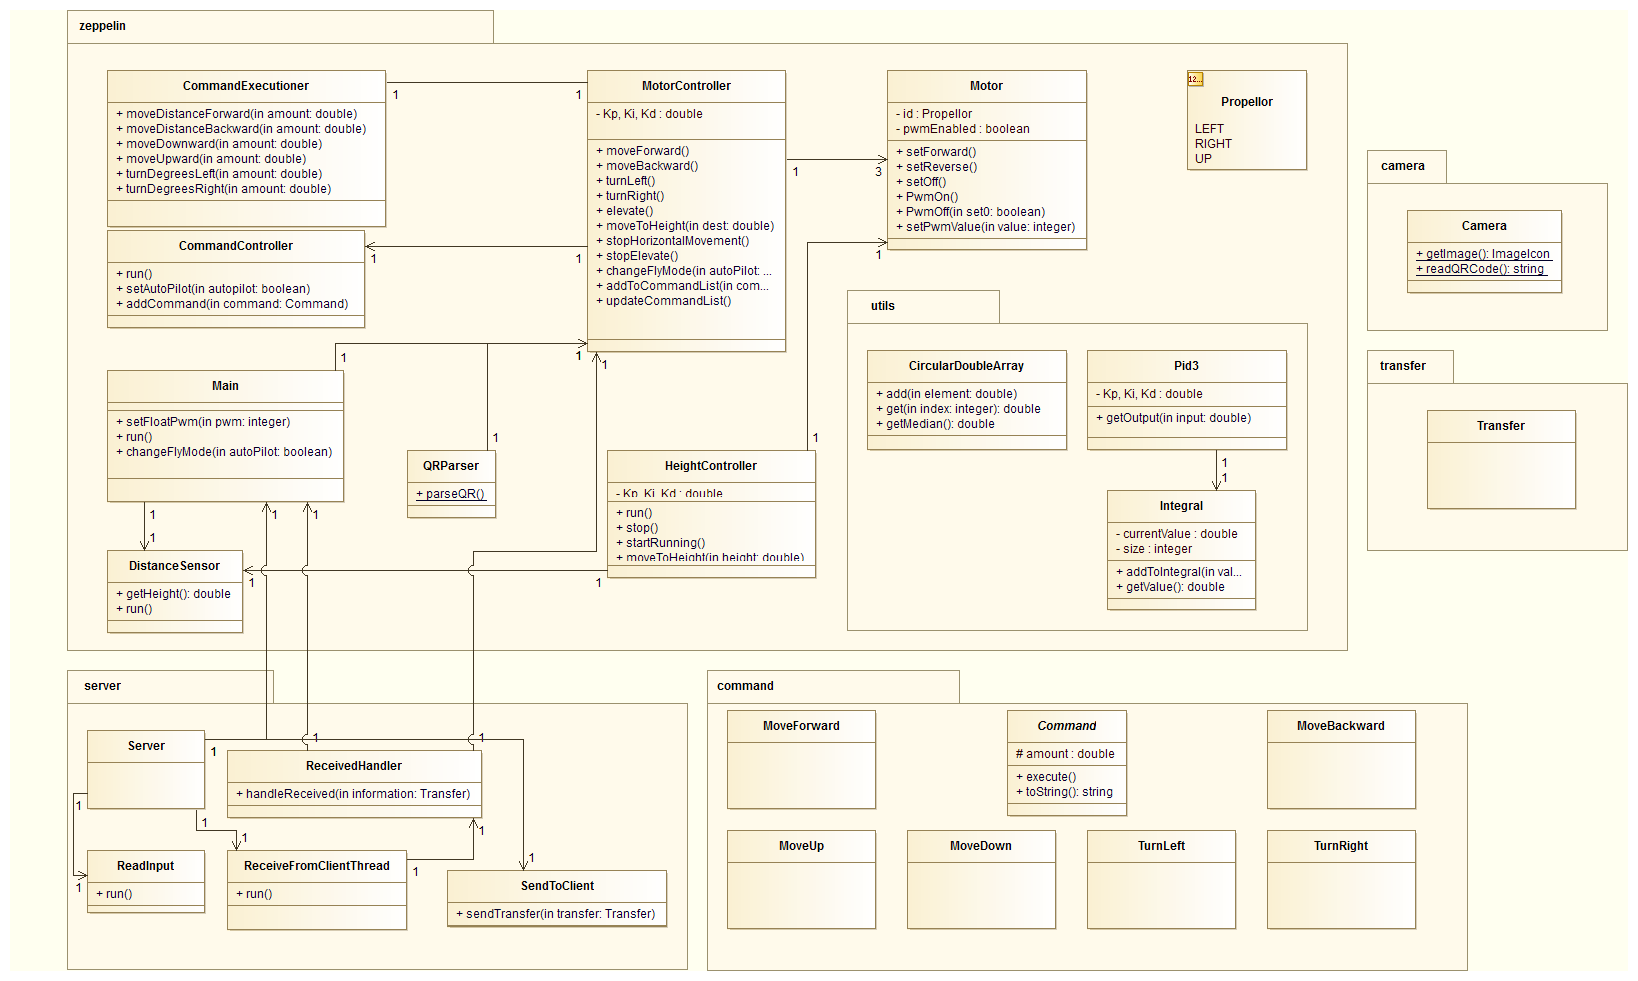
\includegraphics[scale=0.4, angle=90]{UML.png}
\caption{Klassediagram van de interne programmatie}
\label{UML}
\end{figure}

% == GUI == %
\section{GUI}
De User Interface stelt de gebruiker in staat om vanaf een client-pc verbinding te maken met de zeppelin. De GUI geeft informatie weer over de status, zoals de huidige hoogte en commando's die worden uitgevoerd. Daarnaast kan de gebruiker de zeppelin aansturen via de pijltjestoetsen. \\

De eerste tab ('main') toont de hoogte en toestand van de propellers. Er is ruimte voorzien om foto's (van de camera) te tonen en om de commando's weer te geven die in de wachtrij van de zeppelin zitten. Verder zijn hier toetsen om de motoren aan te sturen en om de zeppelin naar een bepaalde hoogte te laten stijgen.\\

De tweede tab geeft een uitgebreider overzicht van de informatie die wordt uitgewisseld tussen de GUI en zeppelin, met een indicatie van de tijd. \\

De zeppelin (server) staat slechts toe dat er \'e\'en client verbindt, dus dat er \'e\'en GUI wordt getoond. Het zou mogelijk zijn meerdere clients toegang te geven, maar om conflicten (met pijltjestoetsen) te vermijden en om bandbreedte te besparen (bij het doorsturen van afbeeldingen), ondersteunt de server maar 1 client. \\

\begin{figure}[ht!]
\centering
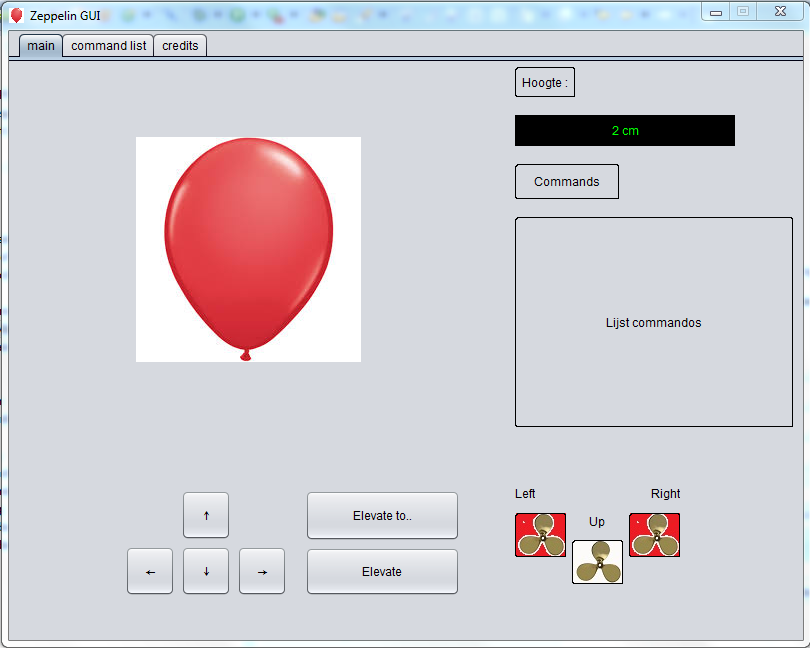
\includegraphics[height=40mm]{GUI.png}
\caption{GUI}
\label{GUI}
\end{figure}


% == BESLUIT == %
\section{Besluit}
We zijn er tot nu toe in geslaagd een zeppelin in elkaar te steken en de motoren aan te sturen. Via sockets wisselen we informatie uit tussen de zeppelin en de GUI en kunnen we de zeppelin via de pijltjestoetsen aansturen. Verder toont de zeppelin op de GUI zijn status en afbeeldingen aan de gebruiker. \\

Naar de toekomst toe moeten we de interne programmatie van de zeppelin verder uitbreiden, zodat hij een bepaalde afstand kan bewegen of over een bepaalde hoek kan draaien. Hiervoor gaan we veel informatie uit testen moeten gebruiken. Daarnaast zal de zeppelin in staat moeten zijn QR-codes te lezen en te interpreteren, maar hiervoor hebben we al een goede aanzet qua programmatie.



% == APPENDICES == %
\newpage\makeappendix

\section{Beschrijving van het proces}
\begin{itemize}
\item \textbf{Welke moeilijkheden heb je ondervonden tijdens de uitwerking?} \\
Over het algemeen is de uitwerking redelijk vlot verlopen, de zeppelin vliegt en doet wat de tussentijdse demo verlangde.  Kleine problemen bestonden uit het niet direct aanwezig zijn van alle hardware, waardoor we tijdens de beginfase veronderstellingen moesten maken over hoe deze in de praktijk zou werken. Hierdoor moesten we soms op enkele beslissingen terugkomen. De praktijk voldeed dus (zoals we wel hadden verwacht) niet volledig aan de theorie. Dit was goed duidelijk bij het naar links of rechts draaien van de zeppelin. In theorie zou deze op eenzelfde plaats moeten blijven hangen boven een bepaald punt, maar dit was niet het geval. Dit is een klein voorbeeld van een probleem dat we dan door veel testen zullen moeten oplossen. \\
Een ander probleem dat we vooral in het begin hadden, was de communicatie tussen de zeppelin en de GUI. Dit is echter een probleem waarmee alle groepen te maken hadden.\\
Een probleem dat we nu nog ondervinden, is de interferentie tussen de neerwaartse motor en de afstandssensor. Als de motor wordt ingeschakeld, vertonen de meetwaarden van de afstandssensor deviant gedrag. Om dit op te lossen, gaan we het frame aanpassen. 
\item \textbf{Welke lessen heb je getrokken uit de manier waarop je het project hebt aangepakt?} \\
Dat veel testen in de praktijk noodzakelijk zijn. Dit wisten we eigenlijk al maar was bij het opstijgen eens zo duidelijk. De ballon voldeed in het begin vaak niet aan onze verwachtingen (zoals hierboven reeds vermeld). Ook was goed plannen en op tijd aan het schrijven van software/testen van hardware beginnen een goede les, onvoorziene problemen kunnen daardoor opgelost worden. \\
Op het vlak van rapporteren hebben we vooral geleerd dat we veel moeten motiveren. We mogen ook niet verwachten dat de lezer even goed als wijzelf op de hoogte is van de details van het project.
\item \textbf{Hoe verliep het werken in team? Op welke manier werd de teamco\"ordinatie en planning aangepakt?} \\
Het werken in team verliep zeer vlot, tot bijna perfect. Iedereen was leergierig en bereid veel tijd te investeren in het project. Het enige minpunt was dat er soms niet genoeg werk was voor iedereen waardoor er af en toe met 2-3 personen aan 1 computer gewerkt moest worden. \\
De eerste les hebben we een teamco\"ordinator en secretaris gekozen, maar deze keuzes waren eerder gemaakt omdat we toen nog geen idee hadden hoe het project ging verlopen. Een co\"ordinatorrol was eigenlijk niet nodig, er werd goed tussen de verschillende groepsleden gecommuniceerd en bij problemen kon je terecht op de Facebook-groep die we hebben aangemaakt. De rol van secretaris hebben we allemaal gedeeltelijk ingevuld: wie even geen taak had, kon aan de verslagen werken, die dan nadien door alle groepsleden nagelezen en aangepast werden. \\ 
Tijdens de eerste 2 lessen werd het al duidelijk welke grote delen er geprogrammeerd moesten worden. Hiervoor hebben we dan een aantal personen per deel gezet.  Meer hierover is in het volgende deel terug te vinden.

\end{itemize}


\section{Beschrijving van de werkverdeling}
De eerste lessen hebben we besloten dat er 3 grote delen waren die moesten afgewerkt worden: de GUI, de communicatie tussen GUI en zeppelin en de zeppelin zelf. Ook waren er de tussentijdse verslagen en het testen van de onderdelen. \\
\begin{itemize}
\item Wander Bavin: Heeft meegewerkt aan het onderdeel GUI. Dit deel vroeg vooral in het begin wat werk. Nadat de GUI afgewerkt was heeft hij verslagen gemaakt/nagelezen en uiteindelijk meegewerkt aan het motor-gedeelte. Indien er extra informatie op de GUI moest verschijnen heeft hij hiervoor gezorgd. Vervulde de rol van co\"ordinator, maar die was in deze goede groep niet echt nodig.
\item Dimitri Jonckers: Heeft meegewerkt aan het onderdeel GUI. Heeft net zoals Wander de verslagen gemaakt en nagelezen, alsook meegeholpen aan het testen van de afstandsensor en het programmeren van de motoren. Ook hij heeft de GUI aangepast wanneer nodig. Heeft thuis veel opzoekwerk gedaan/geprogrammeerd. Heeft de meeste weekly progress reports geschreven.
\item Sunil Tandan: Heeft gewerkt aan het deel communicatie tussen GUI en zeppelin. Dit was een groot en belangrijk deel dat hij op zichzelf heeft gemaakt. Dit deel vroeg redelijk wat werk en moest elke keer wel een beetje aangepast worden (bijvoorbeeld voor het versturen van images). Heeft elk verslag nagelezen en delen over de communicatie toegevoegd. Nadien heeft hij het werken met de camera op zich genomen.
\item Wout Vekemans: Heeft meegewerkt aan het deel motoren/zeppelin. Tijdens de beginfase voornamelijk verslagen gemaakt/nagelezen. Heeft samen met Vince de afstandssensor getest/geprogrammeerd en is daarna aan de motoren beginnen werken. Hij vervulde de rol van secretaris en stuurde de verslagen dus telkens door.
\item Vince Goossens: Heeft meegewerkt aan het deel motoren/zeppelin. Tijdens de beginfase voornamelijk verslagen nagelezen. Heeft samen met Wout de afstandssensor getest/geprogrammeerd en is daarna aan de motoren beginnen werken/programmeren.
\end{itemize}

Hieronder is een tabel te vinden met de gewerkte uren binnen en buiten de sessies: \\

\begin{tabular}{r||r|r|r|r|r}
Overzicht: & Dimitri Jonckers & Wander Bavin & Wout Vekemans & Sunil Tandan & Vince Goossens \\
\hline \hline 
30/09 - 06/10 & 5 & 5 & 5 & 7 & 5 \\
07/10 - 13/10 & 15.5 & 12 & 6 & 11 & 5 \\
14/10 - 20/10 & 11 & 10.5 & 6.75 & 9 & 6.25 \\
21/10 - 27/10 & 9 & 5.5 & 6 & 9 & 5.5 \\
28/11 - 03/11 & 12 & 5 & 5 & 5 & 5 \\
04/11 - 10/11 & 15 & 16 & 10 & 16.5 & 10 \\
\hline \hline
Totaal & 67.5 & 54 & 38.75 & 57.5 & 36.75 \\
\end{tabular}

\section{Kritische analyse}
De groepssfeer en onderlinge samenwerking was zeer goed, de deadlines voor tussentijdse verslagen en de demo zijn makkelijk behaald. Veel zwakke punten zijn er eigenlijk niet, er werd altijd hard gewerkt om zo snel mogelijk een onderdeel van het project af te werken. Het enige zwakke punt was eventueel de werkverdeling: iedereen wou ergens aan werken maar vaak was iemand anders hiermee al begonnen. Verbetering bestaat er dan in het werk misschien wat eerlijker te verdelen (wat niet zo makkelijk is als iedereen veel wil doen). We zouden niet veel anders aangepakt hebben, alles verliep vlotjes en we hadden niet veel problemen met software of hardware.



\end{document}
